\subsection{Signed mass measurements enable calibrated semantic repair}
\label{sec:mnist}
Signed regional measurements distinguish missing probability from excess
probability (Supp.~Sec.~H.2).
In MNIST~\cite{lecun1998mnist}, withholding digit~3 creates persistent
real-data-relative depletion under DDIM25, DDIM50, and DPM++25 in all three
training seeds. Two calibrated classifiers define consensus digit regions
and rejection; accepted real-image accuracy is 99.916\%, and rejection
remains in every probability denominator. The original comparison spans
three training seeds, five training states, and eleven samplers (165
evaluations); its paired restoration contrast uses the frozen
three-comparison adjustment. At DPM++25, ordinary restoration
raises digit-3 mass from 0.00087 to 0.08747, toward the data target 0.0983;
the adjusted paired increase is 0.08660 [0.07677,0.09643]. Coverage rises
from 0.727 to 0.777. Precision drops by 0.01407 versus continued withholding,
while the declared five-percentage-point fidelity margins pass against the
full-data control. Doubling the restored digit's training weight overshoots
to mass 0.1618.

To test whether ordinary training repairs the overshoot, the follow-up
compares 8,000 ordinary-data and 8,000 continued-targeting
updates from identical model, optimizer, EMA, and random states.
Each arm receives 16,000 diagnosis and 2,000 independent outcome samples.
Class-mass error averages the absolute real-to-generated probability
differences across the ten accepted digit regions.
On DPM++25 outcomes, it falls from 0.02177 to 0.00900 (58.7\%),
with paired difference $-0.01277$ [$-0.01878,-0.00676$]. Digit-3 absolute
error falls from 0.06837 to 0.00747 (89.1\%):
$-0.06090$ [$-0.11814,-0.00366$]. The two prespecified 97.5\% paired Student-$t$ intervals
use three training seeds and condition on the shared data reference.
All four fixed-reference precision and consensus fidelity constraints pass.
The ordinary continuation's classifier acceptance is 87.4\%, compared with
95.5\% on real data and 87.3\% for the full-data control.
The ordinary and targeted continuations put 9.08\% and 16.67\% of
outcome images in the digit-3 region, respectively, against 9.83\%
in the real reference. Both error reductions also hold descriptively
under DDIM25 and DDIM50 (Supp.~Sec.~H.2).
Digit-3 equivalence within $\pm0.03$ holds in all nine ordinary-continuation
seed--sampler probes; all-class equivalence and coverage superiority remain
unresolved. Diagnosis costs 48,000 images and 1.6 million denoiser calls
per checkpoint across the three probes.

The same fresh outcomes support a secondary check that includes rejection.
Each image belongs to one of ten consensus digit regions or the reject
region. We compute total variation for each branch and seed as half the
sum of the eleven absolute probability gaps to real data.
It falls from 0.1461 to 0.0854 on average, a 41.6\% reduction,
with paired difference $-0.0608$ [$-0.0828,-0.0387$] (Fig.~\ref{fig:mnist-full-balance}).
The full-distribution improvement holds in all three seeds even though
rejection remains elevated relative to real data. This secondary analysis
uses classifier events from the same paired outcomes.

\begin{figure}[t]
\centering
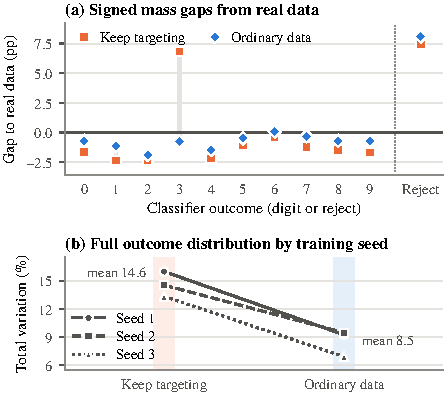
\includegraphics[width=\linewidth]{../figures/mnist_full_balance.pdf}
\caption{Ordinary continuation reduces imbalance across the complete
set of classifier outcomes. (a) Mean signed probability gaps to the
fixed real reference, in percentage points, include the reject event
(R). (b) Lines connect paired total variation estimates for the three
training seeds at the same 8,000-update budget and with 2,000 fresh
images per branch and seed. The secondary paired interval in the text
is a descriptive 95\% Student-$t$ interval.}
\label{fig:mnist-full-balance}
\end{figure}

The CIFAR-10 semantic check uses ten accepted classes plus rejection;
real-image consensus acceptance is 90.75\%, with 98.75\% accuracy among
accepted images. With one adaptation seed and 3,000 matched updates, ordinary
continuation improves DPM25 KID from 0.01479 to 0.01010 and ten-region
mean absolute mass error from 0.0247 to 0.0148. It improves both outcomes
under all five samplers and passes the declared precision/acceptance
constraints. Event-ratio weighting is worse on both metrics under all three
long-step probes. These descriptive controls show how regional measurements
and matched updates distinguish an effective continuation from a targeted
intervention whose additional benefit is unresolved.

Reference refinement supplies a further control before attributing regional
imbalance to training. The accepted frog-region mass changes from 0.138
under DPM++25 to 0.103 under DDIM200, against 0.0943 in observed data.
A separately fitted DINO classifier reproduces the direction. These fixed-event
descriptive measurements show why persistence across qualified sampler probes
is part of the training comparison: a discrepancy that shrinks with the
reference sampler is not, by itself, evidence of persistent data imbalance.

\subsection{Crossed probes separate sampler deficits from persistent depletion}
\label{sec:crossed-probes}
A short sampler can create a regional deficit that clears when
sampling is given more steps. We tested this by crossing two short samplers and three
resolved probes with five MNIST training states and three seeds
(Supp.~Secs.~H.3--H.4). Each short sampler was compared with a
25-call reference from the same checkpoint. To recommend a training
test, we also required the same real-data-relative deficit to persist
under all three resolved probes, each passing its fidelity gates.
The resulting recommendations were frozen before outcome generation.

All 12 short-sampler cases from the two withheld training states
retained digit-3 depletion under the three resolved probes and received
both recommendations. The other 18 cases received a sampler test.
An occupancy-only rule would also have flagged nine of these 18 for
training. On fresh samples, the 25-call sampler improved class-mass
error, coverage, and classifier acceptance in all 18, with a precision
loss relative to the four-call sampler. This comparison increases
inference cost from two or four calls to 25. It also leaves open
whether training could further help. Targeted checkpoints, for example,
still overrepresent digit~3, which the depletion rule does not test.

On the six cases starting from the original withheld state, combining
ordinary restoration with the resolved sampler raises digit-3 mass
to 0.08567, compared with 0.00067 for the resolved sampler with
continued withholding. Both branches use the same training update
budget. The mean class-mass error difference is $-0.00331$
[$-0.00683,0.00020$], an ordinary paired 95\% interval across three
training seeds after averaging the two short settings within each seed.
The crossed test identifies persistent depletion, while the independent
outcomes show which repair objectives improve under the chosen comparison.
